\subsubsection{Zweifach-Fung Effect}
\noindent For several decades, extensive \textit{in vivo}\cite{FungYuan-Cheng1973Sfic, SVANES1968210, PRIES198981}, \textit{in vitro}\cite{Bugliarello469, Roberts2003, Roberts2006, doyeux_podgorski_peponas_ismail_coupier_2011, Zhou2021EmergentBifurcations}  and theoretical\cite{PriesA.R1996Baob, PriesAR1990BFiM, YAN199117, Balogh2018, Freund2014, wang_sui_salsac_barthes-biesel_wang_2016, wang_sui_salsac_barthes-biesel_wang_2018, Barber2011SimulatedPartitioning, Xiong2012Two-dimensionalEffects, 2020Charles} studies have been conducted to comprehend the cell trajectory and path selection of single/multiple RBCs at bifurcations. It is well-recognised that the RBC volume concentration (i.e. haematocrit) in both child branches of a bifurcation is frequently not partitioned equally because of the particulate nature of RBCs. Observations have shown that the fractional RBC fluxes (Q$^{*}_{rbc}$) each child branch receives at a given bifurcation can be greater or lesser than the fractional blood flow rates (Q$^{*}_{blood}$).\cite{Liu2020HeterogeneousBifurcations, doyeux_podgorski_peponas_ismail_coupier_2011, PriesA.R1996Baob, LIPOWSKY1977345} The fractional RBC fluxes increases in the child branch with the higher blood flow rate, whereas the fractional RBC fluxes decrease (even reaching zero) in the child branch with the lower blood flow rate. This phenomenon is known as the Zweifach-Fung effect\cite{SVANES1968210} which also refers to the heterogeneous partitioning of RBCs in the microvascular network. \\

\noindent For blood flow modelling in micro-vascular networks, numerous numerical results of idealised\cite{DominikObrist2010Rbcd, Balogh2018, Balogh2017DirectNetworks} or realistic\cite{2020Charles} micro-vascular networks have shown heterogeneous RBC distribution even if the network is symmetrical. An example is a recent study by Balogh and Bagchi\cite{Balogh2017DirectNetworks, Balogh2018} who have developed a direct numerical simulation technique and demonstrated how RBC partitioning can fluctuate between classical and reverse partitioning over time. These are the two possible outcomes of disproportionate partitioning observed in many studies. Classical partitioning occurs when the child branch with a greater fractional blood flow (Q$^{*}_{blood}$) receives an even greater fractional RBC flux (Q$^{*}_{rbc}$) and vice versa [i.e. Q$^{*}_{rbc}$ $>$ Q$^{*}_{blood}$ when Q$^{*}_{blood}$ $>$ 0.5 and Q$^{*}_{rbc}$ $<$ Q$^{*}_{blood}$ when Q$^{*}_{blood}$ $<$ 0.5]. Unlike classical partitioning, reverse partitioning was also observed in prior studies\cite{ShenZaiyi2016Iohp, PRIES198981, SCHMIDSCHONBEIN198018, Sherwood2014} and it occurs when the child branch that gets the higher fractional blood flow (Q$^{*}_{blood}$) actually gets a lower fractional RBC flux (Q$^{*}_{rbc}$) [i.e. Q$^{*}_{rbc}$ $<$ Q$^{*}_{blood}$ when Q$^{*}_{blood}$ $>$ 0.5 and Q$^{*}_{rbc}$ $>$ Q$^{*}_{blood}$ when Q$^{*}_{blood}$ $<$ 0.5]. This allows us to observe and study the RBC partitioning at each bifurcation in microvascular networks for both \textit{in vivo} or \textit{in silico} experiments. 


% \noindent A correlation between the RBC reverse partitioning and the skewness of the haematocrit profile due to sequential converging and diverging bifurcations was reported in a recent computational study.\cite{Balogh2018} \\


\subsubsection{Plasma Skimming Effect}
\noindent Plasma skimming is a steady-state phenomenon in accordance with the advection of a haematocrit profile by the fluid velocity field through a bifurcation.\cite{YAN199117, EndenG1994ANSo} As mentioned in Section \ref{InitialRBCDistributionInPB}, several established models\cite{PRIES198981, GuibertR2010ANAt, Gould2015HematocritNetworks, LeeTae-Rin2017Gpsm} have been developed to quantitatively describe the plasma skimming effect which underlines the hydrodynamics of disproportionate partitioning in micro-circulations. One widely-applied model is the Phase-Separation Model developed by Pries et. al.\cite{PriesAR1990BFiM, A.R.Pries2005Mbvi} through \textit{in vivo} experiments and theoretical modelling. The non-uniform haematocrit profile at the inlet of a diverging bifurcation was the cause for plasma skimming effects to occurs which results in a disproportionate partitioning of RBCs downstream. This applies to a whole vascular network level as well, given that when the haematocrit profile is advected, the development of the RBC distribution ahead of each bifurcation across the network was found to be uneven.\cite{Balogh2017DirectNetworks} However, results from Balogh and Bagchi studies have demonstrated that plasma skimming was not the only contributing factor that accounts for the full extent of disproportionate partitioning as the other contributing factor to phase separation was the cell screening effect. On top of this, their observations have shown that a more focused haematocrit profile would lead to a broader range of disproportionality within a vessel segment especially for smaller diameter vessels.\cite{Balogh2018} Therefore, this indicates that the partitioning behaviour in each bifurcation is determined by the skewness of the haematocrit profile on average. 



\subsubsection{F{\aa}hr{\ae}us-Lindqvist Effect}
\noindent From the original works of F{\aa}hr{\ae}us and Lindqvist\cite{Fahrus1931THETUBES}, many studies\cite{Pries1992BloodHematocrit, Possenti2019, A.R.Pries2005Mbvi, VahidkhahKoohyar2016FoRB, Adjoua2019, McKayC.B1988OFaF, PRIESA.R1998Saas} have been carried out to understand and quantify the non-continuum effects of blood flow on the flow resistance of a micro-vessel. The apparent viscosity of blood was conveniently used to describe the rheological effects associated with RBCs in the micro-vessels. Based on the numerous experiments of passing human blood through a variety of narrow glass capillary tubes with different diameters, a consistent finding was observed where the apparent viscosity decreases significantly with decreasing tube diameter below around 300 $\mu$m. This phenomenon is known as the F{\aa}hr{\ae}us-Lindqvist Effect\cite{Fahrus1931THETUBES} and the tendency of RBCs to migrate away from the interior wall of the vessels is largely responsible for this effect.\cite{goldsmith1971red, goldsmith1989robin}

\begin{figure}[H]
\centering
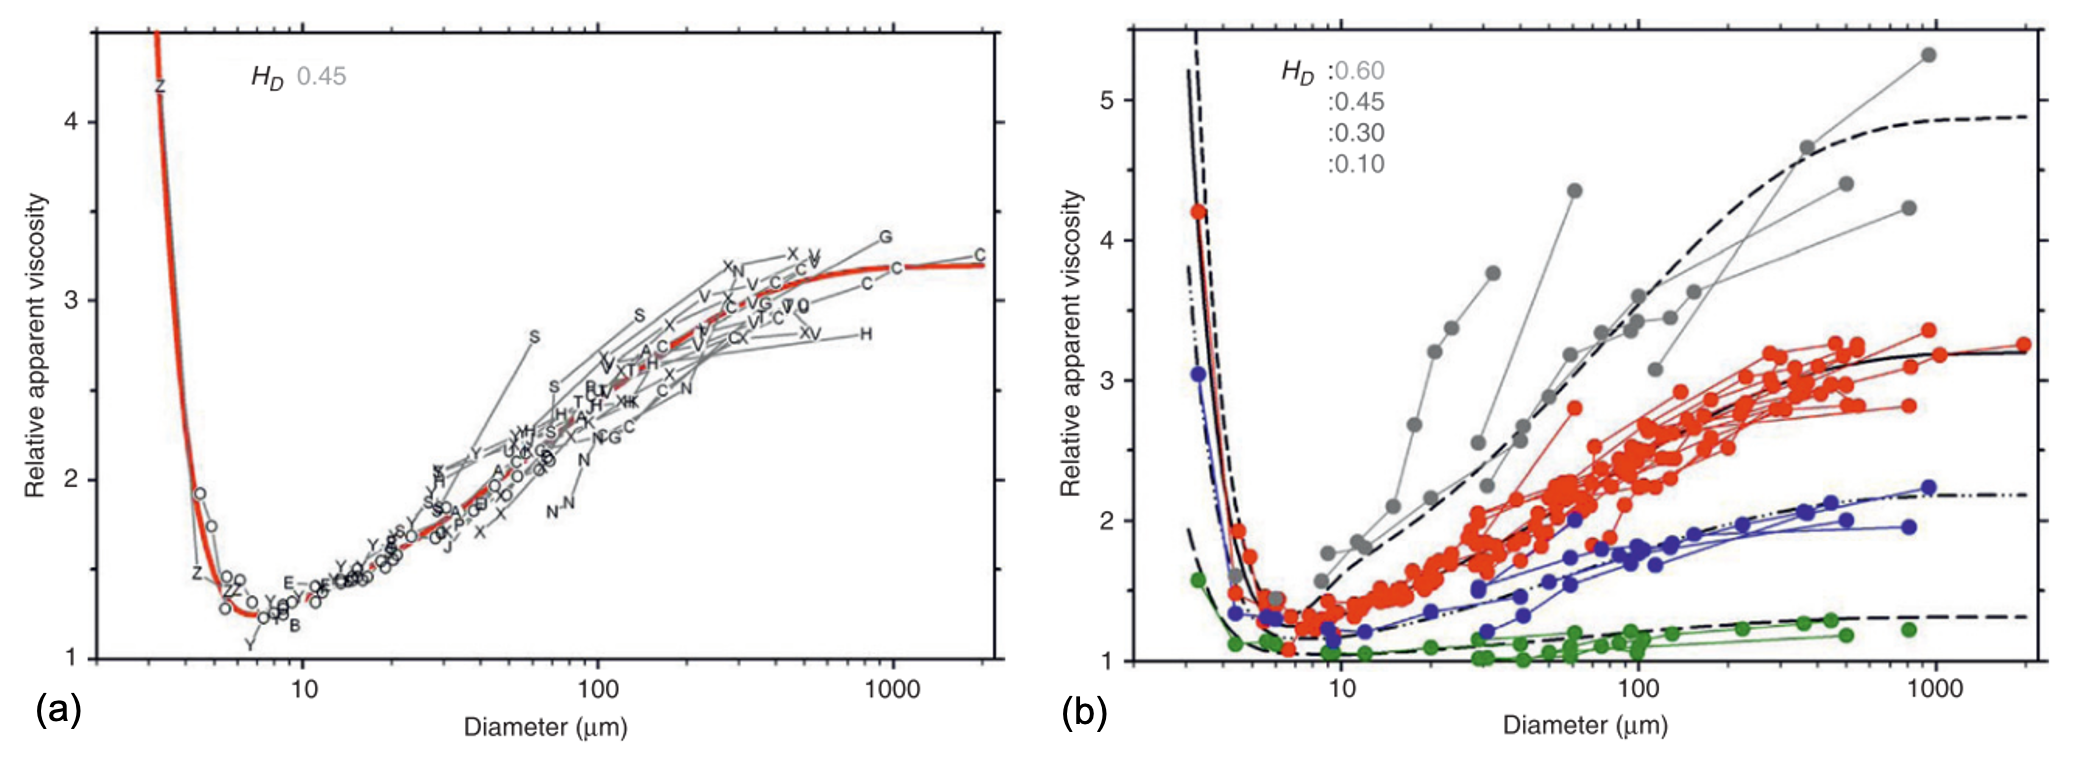
\includegraphics[width=1\textwidth]{images/ApparentViscosity.png}
\caption{\textit{An illustration of all experimental data including empirical lines based on results of parametric fittings. (a) represents the relative apparent viscosity expressed as a function of tube diameter at a discharge haematocrit of 45\%. (b) represents a collection of experimental data and approximations for different levels of discharge haematocrit. H$_{D}$: 0.6 (grey); H$_{D}$: 0.45 (red); H$_{D}$: 0.3 (blue); H$_{D}$: 0.1 (green)} \label{ApparentViscosity}}
\end{figure}

\noindent A comprehensive collection of all the experimental and theoretical results was put together into a graph (see Figure \ref{ApparentViscosity}) by Pries et al.\cite{Pries1992BloodHematocrit, BloodFlowSecomb} The results show that between 5$-$7 $\mu$m, apparent viscosity will reach its minimum before increasing further with decreasing diameter as this also applies to different haematocrit levels.\cite{Pries1992BloodHematocrit} Furthermore, it is expected that the apparent viscosity will increase with the increase of discharge haematocrit at any given diameter. However, between 5$-$7 $\mu$m, it was observed that even at higher haematocrit levels, the relative apparent viscosity remains below 1.5. This suggests that within this range, the presence of RBCs does not have much effect on the flow resistance on glass tubes. \\


\noindent Another important note is that according to these results in Figure \ref{ApparentViscosity}, the apparent viscosity of blood in living micro-vessels tend to be greater than its value in glass tubes with the same diameter. This is primarily due to the existence of endothelial surface layer (ESL) which impedes plasma flow and disrupts the flow of plasma and RBC along the micro-vessel.\cite{Pries2000TheLayer} Therefore, the flow resistance across micro-vessels observed in \textit{in vivo} studies are generally higher compared to that in capillary glass tubes in \textit{in vitro} studies. 